\tikzsetnextfilename{figures/pipelinemodelo/pipelinemodelo}
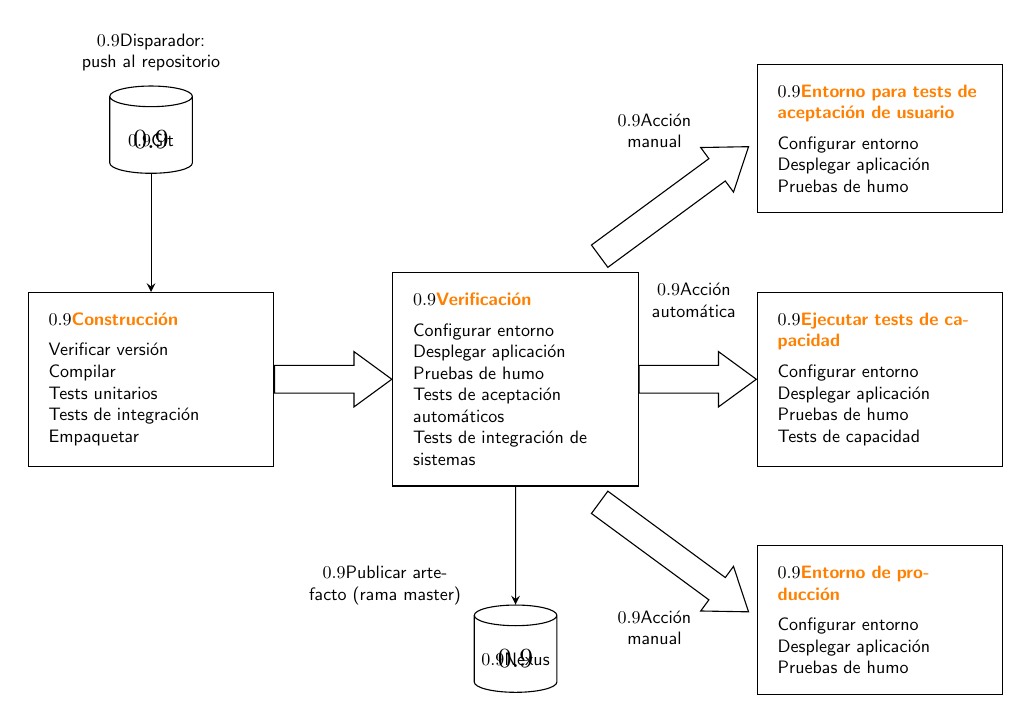
\begin{tikzpicture}[
    font=\relscale{0.9}\sffamily,
    node distance=4cm
  ]

\usetikzlibrary{positioning}
\usetikzlibrary{shapes}
\usetikzlibrary{calc}
\usetikzlibrary{decorations,decorations.text} %  decorations.text just 4 fun

\def\pipelinestage#1#2#3#4{
\node [
  draw,
  rectangle,
  #3,
  scale=0.65,
  text width=4cm,
  inner sep=4mm
] (#2) {
  \textcolor{orange}{\textbf{#1}}
  \smallskip
  \list{}{\topsep=2pt\itemsep=0pt\parsep=0pt
  \parskip=0pt\labelwidth=0pt\leftmargin=0pt
  \itemindent=0pt\labelsep=2pt}
  #4
  \endlist
  };
}

% para poser usar above=of
\begin{scope}[node distance=1cm and 1.5cm]
\pipelinestage{Construcción}{build}{
}
{
  \item Verificar versión
  \item Compilar
  \item Tests unitarios
  \item Tests de integración
  \item Empaquetar
}

\pipelinestage{Verificación}{test}{%
right = of build
}
{
\item Configurar entorno
\item Desplegar aplicación
\item Pruebas de humo
\item Tests de aceptación automáticos
\item Tests de integración de sistemas
}

\pipelinestage{Ejecutar tests de capacidad}{capacity}{%
right = of test
}
{
\item Configurar entorno
\item Desplegar aplicación
\item Pruebas de humo
\item Tests de capacidad
}

\pipelinestage{Entorno para tests de aceptación de usuario}{ua}{%
above = of capacity
}
{
\item Configurar entorno
\item Desplegar aplicación
\item Pruebas de humo
}

\pipelinestage{Entorno de producción}{production}{%
below = of capacity
}
{
\item Configurar entorno
\item Desplegar aplicación
\item Pruebas de humo
}
\end{scope}


\begin{scope}[
node distance=1.5cm,
cylinder,
shape border rotate=90,
aspect=0.25,
shape aspect=0.25,
inner sep=3mm
]
\node[draw,above = of build] (git) {};
\node[draw,below = of test] (nexus) {};
%     \node[annot,above of=N-\hiddenbegin, node distance=1cm] (hl) {Capa oculta};
%     \node[annot,left of=hl] {Capa de entrada};
\end{scope}


\tikzstyle{annot} = [
text width=3cm,
text centered,
node distance=0.1cm,
scale=0.65
]

\node[annot, above= of git] {Disparador: push al repositorio};
\node[annot, above left = of nexus] {Publicar artefacto (rama master)};

\node[annot] at (git.center) {Git};
\node[annot] at (nexus.center) {Nexus};

% https://tex.stackexchange.com/questions/432138/automatically-positioning-node-shape-on-to-path-in-tikz-for-outlined-transpa/432143#432143

\pgfkeys{/tikz/.cd,
    outlined arrow width/.store in=\OutlinedArrowWidth,
    outlined arrow width=10pt,
    outlined arrow step/.store in=\OutlinedArrowStep,
    outlined arrow step=1pt,
    outlined arrow length/.store in=\OutlinedArrowLength,
    outlined arrow length=5mm,
}

\pgfdeclaredecoration{outlined arrow}{initial}
{% initial arrow butt
\state{initial}[width=\OutlinedArrowStep,next state=cont] {
    \pgfmoveto{\pgfpoint{\OutlinedArrowStep}{\OutlinedArrowWidth/2}}
    \pgfpathlineto{\pgfpoint{0.3\pgflinewidth}{\OutlinedArrowWidth/2}}
    \pgfpathlineto{\pgfpoint{0.3\pgflinewidth}{-\OutlinedArrowWidth/2}}
    \pgfpathlineto{\pgfpoint{1pt}{-\OutlinedArrowWidth/2}}
    \pgfcoordinate{lastup}{\pgfpoint{1pt}{\OutlinedArrowWidth/2}}
    \pgfcoordinate{lastdown}{\pgfpoint{1pt}{-\OutlinedArrowWidth/2}}
    \xdef\marmotarrowstart{0}
  }
  \state{cont}[width=\OutlinedArrowStep]{
    \ifdim\pgfdecoratedremainingdistance>\OutlinedArrowLength% continue the outlined path
     \pgfmoveto{\pgfpointanchor{lastup}{center}}
     \pgfpathlineto{\pgfpoint{\OutlinedArrowStep}{\OutlinedArrowWidth/2}}
     \pgfcoordinate{lastup}{\pgfpoint{\OutlinedArrowStep}{\OutlinedArrowWidth/2}}
     \pgfmoveto{\pgfpointanchor{lastdown}{center}}
     \pgfpathlineto{\pgfpoint{\OutlinedArrowStep}{-\OutlinedArrowWidth/2}}
     \pgfcoordinate{lastdown}{\pgfpoint{\OutlinedArrowStep}{-\OutlinedArrowWidth/2}}
    \else
     \ifnum\marmotarrowstart=0% draw the arrow head
     \pgfmoveto{\pgfpointadd{\pgfpointanchor{lastup}{center}}{\pgfpoint{-0.5\pgflinewidth}{0}}}
     \pgflineto{\pgfpoint{-0.5\pgflinewidth}{\OutlinedArrowWidth}}
     \pgflineto{\pgfpointadd{\pgfpointdecoratedpathlast}{\pgfpoint{-0.5\pgflinewidth}{0}}}
     \pgflineto{\pgfpoint{-0.5\pgflinewidth}{-\OutlinedArrowWidth}}
     \pgflineto{\pgfpointadd{\pgfpointanchor{lastdown}{center}}{\pgfpoint{-0.5\pgflinewidth}{0}}}
     \xdef\marmotarrowstart{1}
     \else
     \fi
    \fi%
  }
  \state{final}[width=5pt]
  { % perhaps unnecessary but doesn't hurt either
    \pgfmoveto{\pgfpointdecoratedpathlast}
  }
}

%   \fill[green] (-1,0.5) rectangle (2.5,1.5);
%   \draw(A.north west) -- (D.south east); 
%   \draw[decorate,blue,opacity=0.5] (C) to (D);
%   \draw[decorate,red,opacity=0.5,line width=2pt,outlined arrow length=10pt] (A) to (B);
%   \draw[decorate,outlined arrow length=15pt] (A.east) to[out=0,in=-180] (D.west);
%   \fill[decoration={text along path, text={~here is some text inside an arrow},
%   raise=-2.5pt},decorate]
%   (A.east) to[out=0,in=-180] (D.west);


\draw[decorate,decoration=outlined arrow] (build.east) to (test.west);
\draw[decorate,decoration=outlined arrow] (test) to (capacity);
\draw[decorate,decoration=outlined arrow] ($ (test.north east) + (-0.5,0.2) $) to ($ (ua.west) - (0.1,0.1) $);
\draw[decorate,decoration=outlined arrow] ($ (test.south east) + (-0.5,-0.2) $) to ($ (production.west) - (0.1,-0.1) $);

\node[annot] at ($ (ua.west) + (-1.3,0.1) $) {Acción\\manual};
\node[annot] at ($ (production.west) + (-1.3,-0.1) $) {Acción\\manual};
\node[annot] at ($ (capacity.west) + (-0.8,1) $) {Acción\\automática};

\draw[- stealth] (git) to (build);
\draw[- stealth] (test) to (nexus);

\end{tikzpicture}
